\documentclass[12pt]{article} 
\usepackage{amsmath} 
\usepackage[dvips]{graphicx}
\usepackage{multirow} 
\usepackage{multicol}
\usepackage{geometry} 
\usepackage{pdflscape}
\usepackage[labelfont=bf]{caption} 
\usepackage{setspace}
\usepackage[running]{lineno} 
% \usepackage[numbers,sort]{natbib}
\usepackage[round]{natbib} 
\usepackage{array}
\usepackage[table]{xcolor}

\newcommand{\methods}{\textit{Materials \& Methods}}
\newcommand{\SI}{\textit{Appendix}~}

\topmargin -1.5cm % 0.0cm 
\oddsidemargin 0.0cm % 0.2cm 
\textwidth 6.5in
\textheight 9.0in % 21cm
\footskip 1.0cm % 1.0cm

\usepackage{authblk}

\title{Stable motifs delay species loss in simulated food webs}

% - in intro/discussion, make it clear that this is adding a new layer of meaning to differences/changes in species roles rather than trying to put motifs as the best way to predict extinctions.

% Could try Ecology as a general-purpose option?
% Next Theo Bio, then PeerJ. 
% Reviewers: Jon Borrelli, Benno Simmons, Daniel Stouffer, Tim Poisot, Eva Delmas
% Need 3-5 bullet point highlights, submitted as a separate file. 
% No obvious word limits?
% Cover Letter.  The cover letter should explain how the manuscript fits the scope of the journal, and more specifically how it advances the field, while having broad appeal. If the manuscript relates to any previous submission to an ESA journal, that must be explained as well.  Longer submissions those between 30 and 50 manuscript pages) should be accompanied by a detailed justification for the length. There is a required text box for the cover letter.  Uploading a cover letter as an attachment is optional.

% Submitted manuscripts may have been posted to a preprint archive if the papers in the archive are not peer-reviewed, and provided that a link to the published article will be added if the manuscript is accepted by an ESA journal.  Authors should disclose whether such a posting has been made at the time of submission.

% To do: 
% A - rewrite methods and SI methods following email template.
% A - redo analyses, rewrite results and redo figures
% K - extract species body masses and relate explicitly to threshold of 10^-5. Add line justifying threshold in text.
% K - tidy up key code (test_parameters.jl for network creation, simulate_removals.jl for species removals)
% Both - simplify discussion to correspond to new results
% Both - add Speculations & Alternative Viewpoints section (what if we had a different threshold, webs not structured by body-mass, etc.)
% Both - double-check that we've listed author contributions
% A - contact editors with an apology and find out whether we're now a new submission
% A/Both - finish reply


\author{Alyssa R. Cirtwill$^{1\dagger}$, Kate Wootton $^{2}$} 
\date{\small$^1$Department of Agricultural Sciences\\ 
University of Helsinki\\
Helsinki, Finland
\medskip
\small$^2$ Swedish Agricultural University\\
Uppsala, Sweden\\
\medskip
$^\dagger$ Corresponding author:\\
alyssa.cirtwill@gmail.com\\
 }

\renewcommand\Authands{ and }

\begin{document} 
\maketitle 
\raggedright
\setlength{\parindent}{15pt} 

\clearpage
\linenumbers
\begin{spacing}{2.0}

\section*{Abstract} % Up to 350 words for Ecology
    % Currently 213 words.    
    %Intro
    Some three-species motifs (unique patterns of interactions between three species) are both more stable when modelled in isolation and over-represented in empirical food webs. This suggests that these motifs may reduce extinction risk for species participating in them, ultimately stabilizing the food web as a whole. 
    % Methods
    We test whether a species' time to extinction following a perturbation is related to its participation in stable and unstable motifs and assess how motif roles covary with a species' degree or trophic level.
    % Results
    We found that species' motif roles are related to their times to extinction following a disturbance. Specifically, participating in many omnivory motifs (whether in absolute terms, as a proportion of the species' role, or relative to other species in the network) was associated with more rapid extinction, even though omnivory has previously been identified as a stable motif. Participating in the other three stable motifs (three-species chain, apparent competition, and direct competition) was associated with longer times to extinction.
    %Discussion
    While motif roles were associated with extinction risk, they also varied strongly with degree and trophic level. This means that these simpler measures of a species' role may be sufficient to roughly predict which species are most vulnerable to disturbance, but the additional information encapsulated in a motif role can further refine predictions of vulnerability. Moreover, where researchers are \emph{a priori} interested in motif roles, our results confirm that these roles can be interpreted with respect to extinction risk.%If motif roles are already of interest, however, they can also be used to comment on which species are at greatest risk.

\section*{Keywords}

	species roles; disturbance; competition; three-species chain; omnivory

\clearpage
    
\section*{Introduction}

	The connections between food-web structure and the extinction risk of species within the food web have interested ecologists since at least the 1970's~\citep{May1972}. After early findings suggested that a large, randomly-connected network is unlikely to retain all species after small perturbations~\citep{Gardner1970,May1972}, non-random structures that might stabilize food webs (allowing all species to persist) were quickly identified. These structural features include nestedness~\citep{Allesina2012,Sauve2014}, modularity~\citep{Sauve2014,Thebault2010} and skewed distributions of link strengths~\citep{McCann1998,Gross2009,Rooney2012,Wootton2016}.
	
	
	Although important, these global-scale properties (i.e. properties of the network as a whole, see Fig. \ref{motifs}) can mask important differences in  network structure~\citep{Simmons2019} and do not provide information about differences between species within the same network~\citep{Cirtwill2018FoodWebs}. 
	Two networks with the same connectance and similar values of nestedness and modularity may still have quite different meso-scale (i.e., more detailed than global-scale) arrangements of links. 
	These meso-scale structures, described by frequencies of \emph{motifs} (unique patterns of $n$ interacting species), define the local neighbourhood of a focal species and reflect its direct and close indirect interactions (Fig.~\ref{motifs}).
	
	
    In addition to providing species-level information on network structure, there are early indications that some meso-scale structures may tend to stabilize food webs~\citep{Prill2005,Borrelli2015,Monteiro2016}. 
    This possibility is supported by the fact that empirical food webs tend to contain more \emph{three-species chains} and either more \emph{omnivory} (\emph{sensu}~\citealp[]{Thompson2007b}) motifs or more \emph{apparent competition} and \emph{direct competition} motifs than random networks~\citep{Stouffer2007}. 
    These four motifs make up, on average, about 95\% of all three-species motifs in food webs~\citep{Stouffer2010b}. 
    The high frequencies of these four motifs in observed networks suggest that they may be beneficial to the network containing them or, in other words, that more stable motifs appear more frequently in empirical food webs because unstable motifs are more likely to disappear as the species within them go extinct~\citep{Borrelli2015,Borrelli2015a} or links between species are lost~\citep{Tylianakis2010}.

	When modelled in isolation, three species arranged in \emph{three-species chain}, \emph{apparent competition}, \emph{direct competition}, and \emph{omnivory} motifs are more likely to all persist than trios of species arranged in other motifs~\citep{Borrelli2015a}.
	By damping perturbations and maintaining more constant populations of the species participating in them, these `stable' motifs may contribute to the stability of the network as a whole~\citep{Borrelli2015a}. 
    The greater chances of maintaining all species in a stable motif could explain the over-representation of these motifs in empirical food webs if species and interactions in less-stable motifs are more likely to be ``pruned'' from empirical communities over time. We expect that stable structures will endure for longer than unstable ones, and so it is not surprising that stable structures should be over-represented in empirical communities~\citep{Borrelli2015}.


	Given these early indications that some motifs are more stable than others, we may also expect that a species' role-- here defined as the frequency with which it participates in different motifs --could affect its probability of extinction following a perturbation.
	Specifically, we expect that species participating more frequently in the stable motifs identified by~\citet{Borrelli2015a} are less likely to go extinct than species whose roles are dominated by other motifs.
	Testing this hypothesis is complicated by the fact that species' motif roles are not independent of other aspects of fine-scale network structure. 
    In particular, a species' degree (number of predators and prey) is likely to strongly affect its motif role.
    The more interaction partners a species has, the more motifs in can participate in (Fig.~\ref{motifs}).
    This is likely to lead species with higher degrees to participate in a wider variety of motifs as well as participate more frequently in the four common, stable motifs.
    Species with high in-degrees (more prey) are also generally less likely to go extinct, as are species at lower trophic levels~\citep{Cirtwill2018FoodWebs}.
    Any test for a relationship between motif roles and time to extinction should therefore take degree and trophic level into account to avoid confounding these effects.  
    
    
    Here, we investigate the relationship between species roles and extinction risk by simulating the removal of species from simulated networks at stable equilibria. We test 1) whether species' roles are related to their time to extinction following the removal of another species in the network, 2) whether participation in particular motifs (especially the stable motifs described above) is correlated with time to extinction, and 3) whether these correlations are driven by potential relationships between species' participation in various motifs and simpler definitions of species roles (degree, trophic level). Taken together, these tests show that species are generally consistent in their vulnerability to disturbances, regardless of the location in the network of that disturbance, and this vulnerability is shaped by both motif roles and other network parameters.


\section*{Methods}

    \subsection*{Generating networks and extinctions}

    	\subsubsection*{Generating food webs}
    
    		We simulated a suite of food webs based on the probabilistic niche model, which assigns predator-prey links based on the body-mass ratios between individuals of different species~\citep{Williams2000,Delmas2017}. The meso-scale structure of niche-model networks closely mimics that of empirical food webs~\citep{Stouffer2007}. To ensure that we captured a variety of realistic community sizes and structures, we generated networks ranging between 50 and 100 species (in steps of 10) with connectance values between 0.02 and 0.2 (in steps of 0.02). The range of network sizes was chosen to reflect moderately well-sampled empirical webs while working within our computational limits, while the range of connectance values was chosen to cover that observed in most empirical food webs~\citep{Dunne2002}. We generated a total of 100 networks with each combination of parameters, for a total of 6000 networks (\emph{Appendix S1}). All networks were generated using the function "nichemodel" within the Julia language package \emph{BioEnergeticFoodWebs}~\citep{bioenergeticfw,Delmas2017}. If a simulated network contained any disconnected species (species without predators or prey) or disconnected components (a group of species connected amongst themselves but not to the rest of the network), the network was rejected and a new network simulated. Finally, networks where the path lengths between each species and a basal resource could not be resolved (i.e., trophic levels were undefined) were rejected and new networks simulated.
    
  
    		After generating the network structure, we simulated community dynamics using the function "simulate" from the Julia language package \emph{BioEnergeticFoodWebs}~\citep{bioenergeticfw,Delmas2017}. This function uses Lotka-Volterra predator-prey models including density dependence and type 2 functional responses for all species (please see~\citet{Delmas2017} for full details).
    		All non-basal species were designated as vertebrates to ensure a good match between metabolic and predator-prey body-mass ratio values. Metabolic rates in the Lotka-Volterra model are based on each species' body mass (i.e. mass of a single individual). We assigned relative body masses based on each species' trophic level, which was, in turn, calculated based on the food-web structure provided by the niche model. After basal species were assigned a body mass of 1, we used a predator-prey body-mass ratio of 3.065 to calculate the relative body masses of higher trophic levels. We selected this ratio based on the estimate for vertebrates (averaged across ecosystem and metabolic types) in~\citet{Brose2006}. We excluded reported body-mass ratios for invertebrates as these could include parasites and parasitoids, which are generally smaller than their prey, and because interactions among vertebrates are better represented in the food-web literature than interactions involving invertebrates.
    		
    		
    		The persistence of each species in our simulated networks also depends on its population biomass. 
    		We randomly assigned initial population biomasses (i.e. cumulative biomass across all individuals of a species) for each species from a uniform distribution [0,1]. Note that population biomasses and individual body masses are not calculated on the same scale. We then simulated community dynamics for 1000 time steps to obtain an equilibrium community. To ensure that species did not `recover' from unrealistically low biomasses during the simulation, we considered a species extinct if it dropped below an arbitrary threshold biomass of 1$\times10^{-5}$. When simulating initial (ie. pre-perturbation or equilibrium) dynamics, we rejected any network where one or more species dropped below this biomass threshold. Consumers were assumed to have no preferences such that the consumption rate $w_{ij}$ of predator $i$ eating prey $j$ is equal to $\frac{1}{n}$, where $n$ is the number of prey for predator $i$. If the network did not reach an equilibrium with all species persisting for 1000 time steps, a new set of initial population biomasses was applied and the simulation repeated until an equilibrium with all species persisting was obtained.
    		If a stable equilibrium still had not been reached after 100 sets of randomly-assigned initial biomasses, we discarded the network and simulated another to replace it.
    
    
    	\subsubsection*{Calculating species roles}
    
    
    		We were interested in whether species' roles at equilibrium are related to their response to a perturbation, in this case the removal of another species in the network. We defined each species' role as the number of times it appears in each unique three-species motif, following~\citet{Stouffer2012,Cirtwill2015}. Note that each set of three interacting species forms exactly one motif~\citep{Cirtwill2018FoodWebs}. As our focus is on how different motifs might affect extinction risk, we do not consider the different positions species may take within a motif. We expect that appearing more frequently in stable motifs (three-species chain, apparent and direct competition, and omnivory) will correlate with lower extinction risk while appearing more frequently in unstable motifs (those containing two- or three-species loops) will be associated with higher extinction risk.	Note that cannibalistic links were ignored when calculating motif frequencies within a network and species' roles, although they were included when calculating connectance. As well as these 'raw' motif roles, we calculated 'degree-normalized' motif roles for each species by dividing the number of appearances in each motif by the total number of times the species appears in any motif (as in~\citet{Cirtwill2015}; this total is expected to strongly correlate with degree). Finally, we also calculated 'network-normalized' motif roles, defined as the z-score of the number of times a focal species appears in each motif compared to the number of times all species in the network appear in the focal motif.
    		The degree normalisation allows us to test whether trends in stability with motif participation are due to differences in the total number of motifs a species appears in, while the network normalisation allows us to test whether trends in stability with participation in different motifs are related to how unusual each species is within its community context.
    
    
    	\subsubsection*{Perturbing networks}
    
    		After identifying species' roles in the equilibrium networks, we perturbed the networks by removing a single species. After this removal, community dynamics were simulated for 50 rounds of 10 time-steps (500 time-steps total). After each round, any species with a biomass below our threshold of 1$\times10^{-5}$ was considered to have gone extinct and its biomass was set to 0. We recorded the biomass of each species after each round, as well as the round in which any additional extinctions occurred. After 500 time-steps, we reset the network to its original state (including all species). We then removed a new species and again simulated community dynamics. We repeated this process until all species had served as the initial removal.
    		We then calculated the mean time to extinction across all removals as an overall measure of each species' vulnerability (\emph{Appendix S2}). 
    		Time to extinction was highly correlated across removals in all combinations of S and C, indicating that this is a robust measure.


	\subsection*{Statistical Analysis}

        \subsubsection*{Is motif participation related to persistence?}

            We are interested in whether the set of motifs in which a species appears at `equilibrium' is related to its persistence (here defined as time to extinction following the removal of another species). 
            To address this question, we can consider the motif participation role as a whole or the relationships between participation in each motif and persistence. 
            The first approach provides a more holistic view of the relationship between meso-scale structure and extinction risk, while the second may identify specific meso-scale structures with especially strong relationships to persistence.


            \textbf{Motif participation as a whole}

                To test whether motif participation as a whole is related to persistence, we fit a series of PERMANOVAs relating the Bray-Curtis dissimilarity in species' motif participation vectors to their persistence times (see Appendix \emph{S3} for details). 
                Due to computational constraints, we fit one PERMANOVA per combination of network size and connectance (60 combinations). 
                We repeated these sets of PERMANOVAs for each version of motif participation vectors (counts, species-normalised, and network-normalised; 180 PERMANOVAs in total).
                As PERMANOVAs can return false positives if assumptions about the variability of motif participation vectors are not met (see \emph{Appendix S4}), the results of these tests are indicative but not conclusive.


            \textbf{Participation in particular motifs}

                For a more detailed perspective on relationships between motif participation and persistence, we fit linear mixed-effect models including the effect of each motif separately.
                Since the motifs containing loops (two-way interactions or three-species loops) are rare in both empirical systems~\citep{StoufferXXXX} and our simulated networks (means 8.99$\times10^{-4}$\%-2.06\%) and are all unstable when modelled in isolation~\citep{BorrelliXXXX}, we pool these loop-containing motifs into an 'other' group (see \emph{Appendix S5} for details about how each version of motifs were pooled). 
                We considered each stable motif (apparent competition, direct competition, omnivory, and three-species chain) individually.


                For each version of motif participation (count, frequency, or $Z$-score), we fit a  linear mixed-effect model (LMM) of the form:

                \begin{equation}
                    \tau_{i} \approx \alpha_{i} + \delta_{i} + o_{i} + \chi_{i} + \omega_{i} + S_{i}:C_{i} ,
                    \label{eq:persistence_motifs}
                \end{equation}

                where $\tau_{i}$ is the mean time to extinction (persistence) of species $i$,  $\alpha_{i}$, $\delta_{i}$, $o_{i}$, and $\chi_{i}$ are the species' participation in the apparent competition, direct competition, omnivory, and three-species chain motifs (respectively), $\omega_{i}$ is the species' participation in the unstable motif group, and $S_{i}:C_{i}$ is a random effect of the size and connectance of the network to which $i$ belongs.
                This random effect of global network structure controls for differences in mean persistence between, for example, highly-connected and weakly-connected networks. 
                These models indicate whether each motif is positively or negatively correlated with persistence time, and how much variation in persistence time can be explained by each version of motif participation. 
                We fit the LMMs using the R~\citep{R} function `lmer' from the package \emph{lmerTest}~\citep{lmerTest} and calculated variance explained using the function `r.squaredGLMM' from the package \emph{MuMIn}~\citep{MuMIn}.
                
                
                Note that, in the species-normalised motif participation vectors, the frequencies of all motifs must sum to 1 and are therefore not independent. 
                Participation in the count and $Z$-score motifs also may not be independent (e.g., species which participate in especially many interactions may have high counts and $Z$-scores of several motifs).
                To illustrate these potential interdependences, we also present the correlations among all motifs for each version of motif participation, calculated using the function `lmer' as above.
                

        \subsubsection*{Adding context: how does motif participation relate to simple roles?}

            To interpret the results of the analyses above, especially the LMMs, we must bear in mind the potential for motif participation to reflect differences in degree, trophic level, and global network structure. 
            To establish this context, we therefore fit a series of linear models (LMs) relating degree, trophic level, network size, and connectance to each version of the motif role (Appendix \emph{S6}). 
            These LMs also included a random effect of global network structure.
            For ease of interpretation, we once again grouped the loop-containing motifs into an `unstable' group. 
            When using species-normalised motifs, we removed the `other' motifs from the model to avoid a rank-deficient model matrix.
            
            
            To complete this background, we fit a regression of persistence against degree, trophic level, and their interaction, as well as a random effect of global network structure (Appendix \emph{S7}). 
            These regressions are intended only to confirm whether our simulations show the expected increase in persistence with degree and decrease in persistence with trophic level. 


\section*{Results}
	
    \subsection*{Relating overall motif participation to persistence}
    
		Our series of PERMANOVA tests demonstrated that species' overall raw motif roles were correlated with their mean time to extinction across all combinations of species richness and connectance (Table \emph{S1, Appendix S2}). Taken individually, each PERMANOVA was significant (all $p$\textless0.025). Moreover, after applying the correlated Bonferroni correction~\citep{Drezner2016}, all PERMANOVAs remained significant.
		However, these significant results may be false positives since the variability of raw motif roles was not consistent across mean times to extinction for any combination of species richness and connectance (Table \emph{S3, Appendix S2}). 
		Specifically, longer mean times to extinction were associated with significantly more variable roles, and these relationships were stronger in smaller or less-connected networks. 
		This means that there are many roles which are associated with long times to extinction but fewer roles which are associated with short times to extinction.
		After applying the correlated Bonferroni correction~\citep{Drezner2016}, both the ANOVAs testing for non-homogeneous variability of roles and regressions testing for relationships between role variability and time to extinction remained significant.
    
    \subsection*{Relating participation in particular motifs to persistence}
    
        When defining participation based on counts, increased participation in any motif was correlated with longer persistence following species removal (Table S3, \emph{Appendix S8}).
        Regressions against motif participation explained 0.3-2.2\% of variation in persistence time (fixed effects only).
        When defining participation based on frequencies, greater participation in the omnivory and three-species chain motifs was correlated with longer persistence, while greater participation in any other motif was associated with reduced persistence (Table S4, \emph{Appendix S8}).
        However, the amount of variance in persistence time explained by frequencies was extremely low (maximum 0.004; fixed effects only). 
        When defining participation based on $Z$-scores, unusually high participation in any motif was associated with longer persistence (Table S5, \emph{Appendix S8}).
        The amount of variance in persistence explained by trends in $Z$-score participation was lower than that explained by counts but higher than that explained by frequencies (0.3-1.4\%).
        
    \subsection*{Is motif participation related to simpler roles?}    
    
        As expected, a higher degree was associated with higher counts and higher $Z$-scores of any motif (Appendix \emph{S6}).
        A greater frequency of omnivory was also associated with higher degree, while the converse was true for all other motifs.
        Un-normalised (count-based) motifs explained almost all variance in degree, while the correlation between network-normalised ($Z$-score) motif participation and degree was weaker. 
        
    
        The relationships between motif participation and STL were extremely weak for all versions of motif participation (Appendix \emph{S6}).
        Nevertheless, a higher trophic level was associated with higher counts and $Z$-scores of the apparent competition motif, higher counts, $Z$-scores, and frequencies (by implication) of the `other' motifs, and higher $Z$-scores of direct competition.
        While significant, these trends explain so little variation in STL that motif participation and trophic level are likely to convey almost independent information about a species' place in the network.
    
    \subsection*{Is persistence related to simpler roles?}
    
        Simple roles (degree and STL) together explained a moderate amount of variation in persistence ($R^2_m$=0.211, $R^2_c$=0.232).
        Species with higher degrees and lower trophic levels tended to have longer mean times to extinction (Appendix \emph{S7}).
        However, a negative interaction term means that an increase in degree is less beneficial for species with high trophic level (Fig.~\ref{fig:persistence_DegTL}).
    
    
Fig. 1 - PERMANOVA and/or dispersion. Something like we've already got, but with an explanation of why dispersion means it's untrustworthy. May need to be dispersion against persistence.

Fig. 2-4 (or 3 panels) - persistence on y axis, motif on x. Show all 5 motifs (4 stable + other) on same pane.


\section*{Discussion}

    We found that times to extinction were tightly correlated across removals. 
    This suggests that the position of a focal species within a network can affect its risk of extinction following a disturbance regardless of where in the network the disturbance is applied. This result also justifies our use of mean times to extinction across removals as a measure of a species' overall risk.
    Taken together, our results show that motif roles are related to mean times to extinction and that the omnivory motif may have a distinct effect from those of the other stable motifs, at least in body-mass structured vertebrate food webs.
    Testing whether these results hold true for other types of networks (e.g., invertebrate food-webs not structured by body mass) will require alternative simulation approaches; however, the increasing availability of highly-resolved empirical data for interactions among invertebrates~\citep{} should allow researchers to create such simulations and test the generality of our results in the near future.


 	\subsection*{Times to extinction are highly consistent}

		The consistency of species' times to extinction across removals in our simulations suggests that some species are more likely to go extinct than others due to their position within a network.
        This complements other work identifying sets of species which are more vulnerable to extinction due to their traits~\citep{Curtsdotter2011,Ryser2019}. 
		Since the trophic level and degree of the species being removed can also affect which species, if any, go secondarily extinct~\citep{Wootton2016a,Dunne2002}, the properties of both disturbed and non-disturbed species affect the ways in which extinctions can cascade through a food web.
		
		
		The stronger correlation of extinction orders in larger, more-connected networks, as well as the somewhat shorter mean times to extinction in these webs (Fig. S1, \emph{Appendix S1}) may be due to the greater number of short pathways by which an extinction somewhere in the web can affect a focal species. 
		These short pathways are more likely to have strong effects on the population dynamics of species along them than the longer indirect pathways in poorly-connected networks~\citep{Jordan2002,Jordan2006}.
		These stronger effects in turn likely explain why more secondary extinctions in large or highly-connected webs are due to indirect effects rather than direct loss of a prey or predator~\citet{Wootton2016a}. 


	\subsection*{Motif roles relate to extinction risk}

		Overall, our results show that species' motif roles were related to their time to extinction after a disturbance (Table~\ref{overview_table}).
		Participating in more instances of the most stable motifs identified by~\citet{Stouffer2007,Borrelli2015a}, having a greater proportion of the role made up by these motifs, or appearing in significantly more of these motifs than other species in the network were all associated with longer times to extinction. 
		Surprisingly, some unstable motifs were also associated with longer times to extinction.
		The unstable motifs are, however, rare in both empirical food webs~\citep{Stouffer2007} and our simulated networks.
		Differences in participation in these motifs is therefore unlikely to have a large practical effect on species' responses to a disturbance.
        
        
        Part of the apparent benefit of participating in many stable motifs may be due to correlations between motif roles and degree.
        Counts of the stable motifs increased most rapidly with increasing degree, meaning that the relationship between high numbers of stable motifs and species persistence~\citep{Stouffer2007,Borrelli2015a} may be partly due to the beneficial effects of having a high degree~\citep{Cirtwill2016a}.
		That is, while a species which participates in many stable motifs is likely to benefit from damping of population cycles~\citep{Borrelli2015a}, it is also likely to maintain a reasonable number of food sources after a perturbation.
		The positive correlations between all four stable motifs and degree may also explain the greater variability among roles of species with long times to extinction.
		As species wither higher degrees also tend to participate in more motifs, there is a broader set of motif roles available to these species.
		Since high-degree species tend to participate in proportionally more stable than unstable motifs, many of the roles in this broad role-space should be associated with long times to extinction.
		
		
        The relationships between trophic level and the counts or proportions of motifs tended to be weaker, although the $Z$-scores of all four stable motifs, tended to decrease strongly with increasing trophic level.
        Species with higher trophic levels also tended to have shorter mean times to extinction, suggesting that these species could be more susceptible due to being at the tops of longer food chains, participating in motifs that tend to amplify population fluctuations~\citep{Borrelli2015a}, or both.
        The correlations between degree, trophic level, and motif roles make identifying the precise mechanisms behind a species' short or long mean time to extinction difficult.
        The possibility that these measures capture at least some independent information about the risk of secondary extinction, however, suggests that species with multiple `risky' roles (i.e., low degree, participation in many unstable motifs, and/or high trophic level) may be more vulnerable than species with only one of the above.

        
    \subsection*{Omnivory may be an especially informative motif}
	    
        Although there may be many motif roles which promote long times to extinction, not all of the stable motifs are equally likely to be included in such roles.
        While the three-species chain, apparent competition, and direct competition motifs were all associated with longer times to extinction as expected, the omnivory motif was associated with shorter mean times to extinction. 
        This is consistent with an omnivory motif being less likely to retain all three species than the chain, apparent competition, or direct competition motifs when modelled in isolation~\citep{Borrelli2015a}. 


        It may be difficult to isolate the effect of omnivory, however, as the proportion of the omnivory motif in a species' role increased strongly with increasing degree. 
        This relationship could partly explain the variety of earlier work showing that the omnivory can be stable or unstable under different conditions and may or may not increase the overall stability of an entire food web~\citep{McCann1997,Emmerson2004,Borrelli2015a,Monteiro2016}.
        If high-degree species tend to persist for a long time but high-omnivory species are more likely to go extinct, then it may be difficult to predict the outcome for a species with both high degree and a role rich in the omnivory motif.
        However, this relationship does suggest that motif roles may help us to compare risk for species with similar degrees.


	\subsection*{Moving forward with motifs}	

        As motif roles become more common as tools for ecologists wishing to understand how species' positions within networks are related to their traits~\citep{Cirtwill2018EcolLett}, taxonomy~\citep{Stouffer2007}, and position in space or time~\citep{Baker2015}, it is natural to wonder how these roles might relate to a species' response to disturbance. 
        Our results suggest that participation in the three-species chain, apparent competition, and direct competition motifs promote longer persistence after a disturbance, while the omnivory motif may indicate more rapid extinction.
        However, interpreting these trends is complicated by strong relationships between motif roles and degree, which itself promotes longer persistence after a disturbance.
        
        
	    Because relationships between motif roles and degree appear even when considering the proportion of species roles made up by each motif, as in~\citet{Baker2015,Cirtwill2015,Simmons2019}, normalizing motif roles based on the total number of motifs does not control for differences in species' roles due to degree.
	    The papers cited above explicitly aim to control for differences due to the total number of motifs in which a species appears (which depends upon the degrees of the focal species \emph{and} those of its interaction partners) rather than degree \emph{per se}.
	    However, this distinction is subtle (hence our use of `degree-normalization' to describe the proportional roles) and future authors should take great care that they are not using the sum of motifs as a substitute for degree as our results show that these quantities are not interchangeable.
        Rather, our results suggest that both motif roles and simpler measures of network structure can provide information about a species' response to disturbance.
        Motifs may be particularly useful when comparing species with similar  or trophic levels: the multi-dimensional nature of the motif role allows it to capture information which is lost in single-value measures such as degree or trophic level.
        While the interpretation of motif roles remains challenging, the relationships we have found between these roles and time to extinction suggest that they are worth retaining in the toolbox of ecological network analysis.
        

\section*{Acknowledgements}

	We thank Eva Delmas and Chris Rackauckas for their kind assistance with troubleshooting the simulation model and the Spatial Foodweb Ecology Group for providing feedback on the manuscript. ARC is supported by a Finnish Academy Postdoctoral research grant (\#332999). 


\clearpage
    \bibliographystyle{ecollett} 
    \bibliography{MyCollection} % Abbreviate journal titles.

\clearpage
\end{spacing}

% \begin{landscape}
% \section*{Tables}

%     \begin{table}[h!]
%         \centering
%         \footnotesize
%         \caption{Summary of analyses performed and results obtained therefrom. `S' refers to species richness, `C' connectance, `Ext' to mean time to extinction across removals, `STL' to shortest trophic level, and `Deg' to degree (number of interaction partners). }
%         \label{overview_table}
%         \begin{tabular}{m{6cm}|m{7.5cm}|m{8cm}}
%         Question & Test & Result \\
%         \hline
%         Are roles (count) related to Ext? & 
%         \begin{itemize}
%             \item PERMANOVA of Ext vs. role
%             \item one per S-C combination (60 total)
%         \end{itemize} 
%         & \begin{itemize} \item Yes. All PERMANOVA significant. \end{itemize} \\
%         Are roles (count) similarly variable in species with long and short Ext? & 
%         \begin{itemize}
%             \item ANOVA of Disp(role) vs. Ext
%             \item Disp(role) calculated by Betadisper
%             \item one per S-C combination (60 total)
%         \end{itemize}
%         & \begin{itemize} \item No. All ANOVA significant. \end{itemize} \\
%         Do species with long or short Ext have more variable roles? & \begin{itemize}
%             \item LM: Disp(role) vs. Ext
%         \end{itemize} & \begin{itemize} \item Roles variability significantly increases with increasing Ext \end{itemize} \\
%         \hline
%         Which motif counts, proportions, and $Z$-scores are most strongly related to Ext? (see Fig.~\ref{coefficient_sum}). & \begin{itemize}
%             \item PLS: Ext vs. role, S, C, S:C, STL, Deg
%         \end{itemize} & \begin{itemize}\item Ext decreases with omnivory but increases with other stable motifs. \end{itemize}\\
%         \hline
%         How do motifs vary with Deg? \newline(see Fig.~\ref{motif_vs_degTL}) & \begin{itemize} 
%         \item LM: Count vs. Deg 
%         \item LM: Proportion vs. Deg 
%         \item LM: $Z$-score vs. Deg 
%         \item One LM per motif (39 total)
%         \end{itemize} 
%         & 
%         \begin{itemize}
%             \item All counts increase with increasing Deg
%             \item Prop. omnivory increases with Deg, other stable motifs decrease
%             \item All $Z$-scores increase with Deg \end{itemize}\\
%         How do motifs vary with STL? \newline(see Fig.~\ref{motif_vs_degTL}) & \begin{itemize} 
%         \item LM: Count vs. STL 
%         \item LM: Proportion vs. STL 
%         \item LM: $Z$-score vs. STL
%         \item One LM per motif (39 total)
%         \end{itemize} &
%         \begin{itemize}
%             \item All counts increase with increasing STL
%             \item Proportion of stable motifs except omnivory decrease with STL
%             \item $Z$-scores of stable motifs decrease with STL
%         \end{itemize} \\
%         \end{tabular}
%     \end{table}
% \end{landscape}

\clearpage

\begin{spacing}{2.0}
\section*{Figure legends}

    % \begin{figure}[h!]
        % 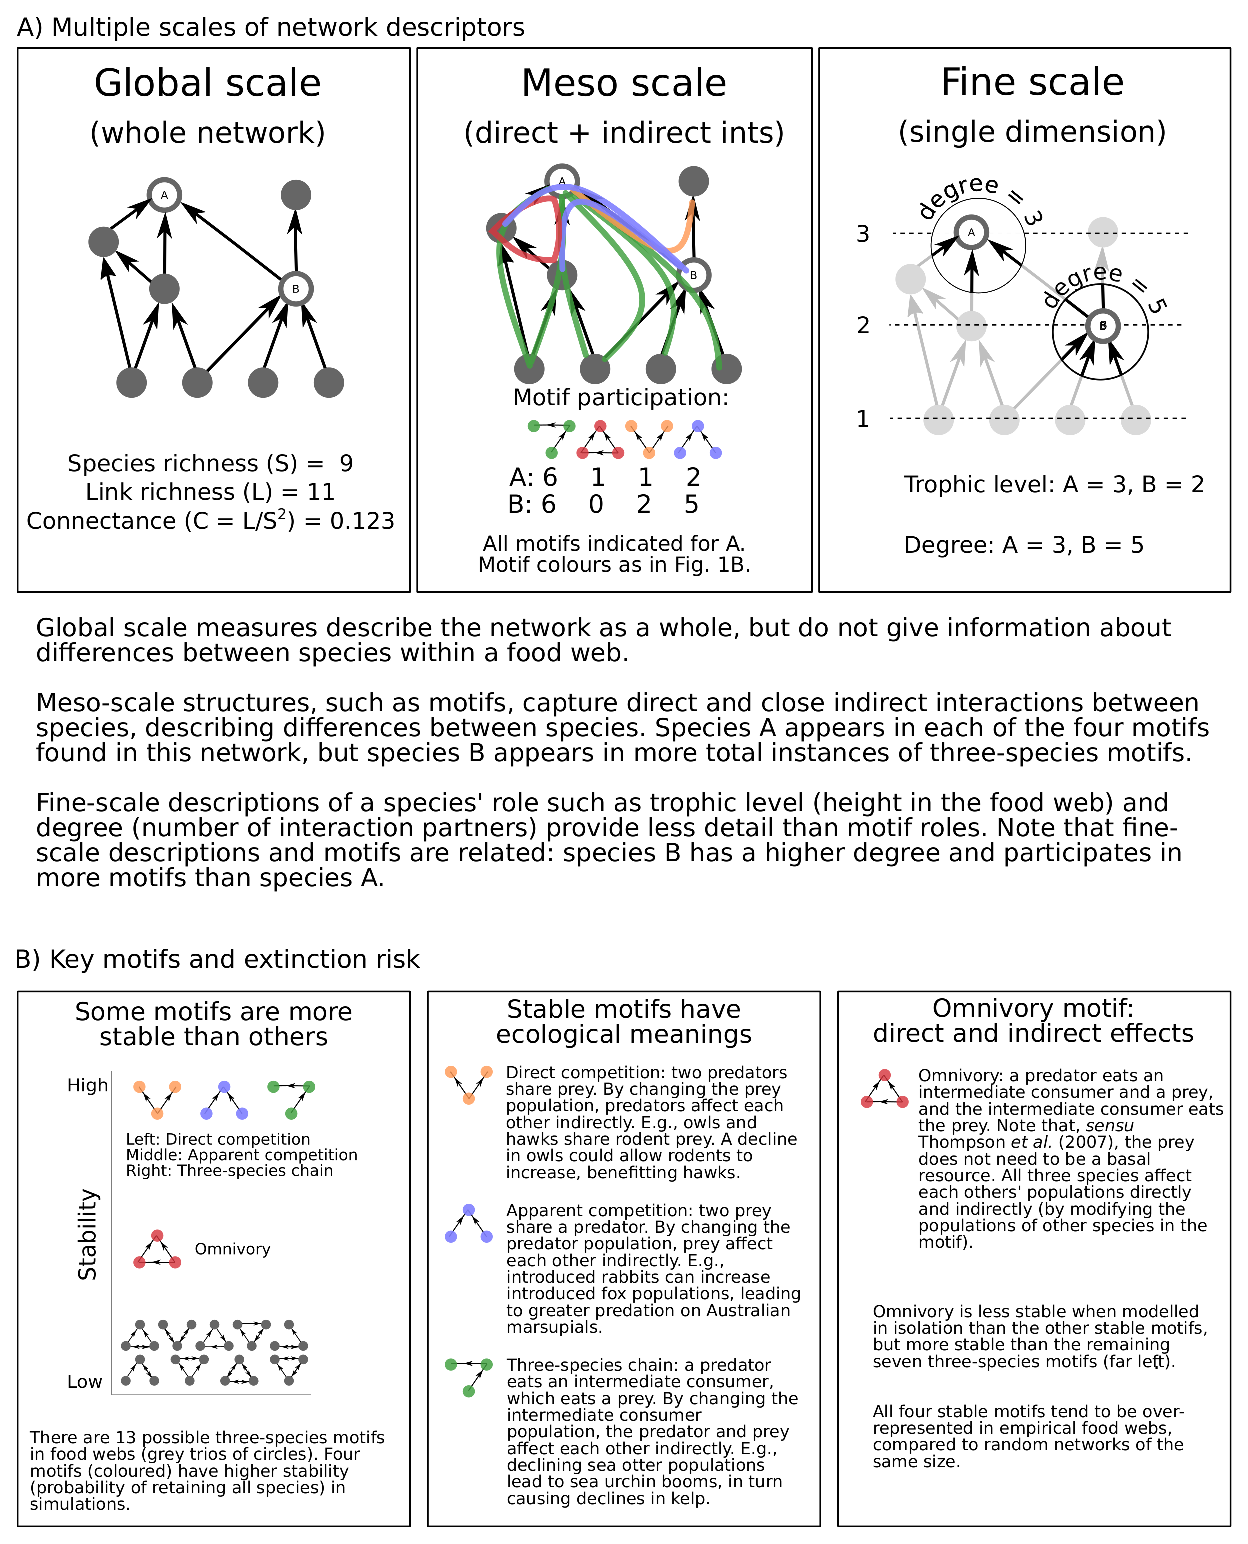
\includegraphics[width=.9\textwidth]{figures/motifs_box.eps}
        \textbf{Figure 1.} A brief introduction to motifs.
        % \label{motifs}
    % \end{figure}

    \vspace{24pt}


\end{spacing}

\clearpage

\section*{Figures}


    \begin{figure}[h!]
        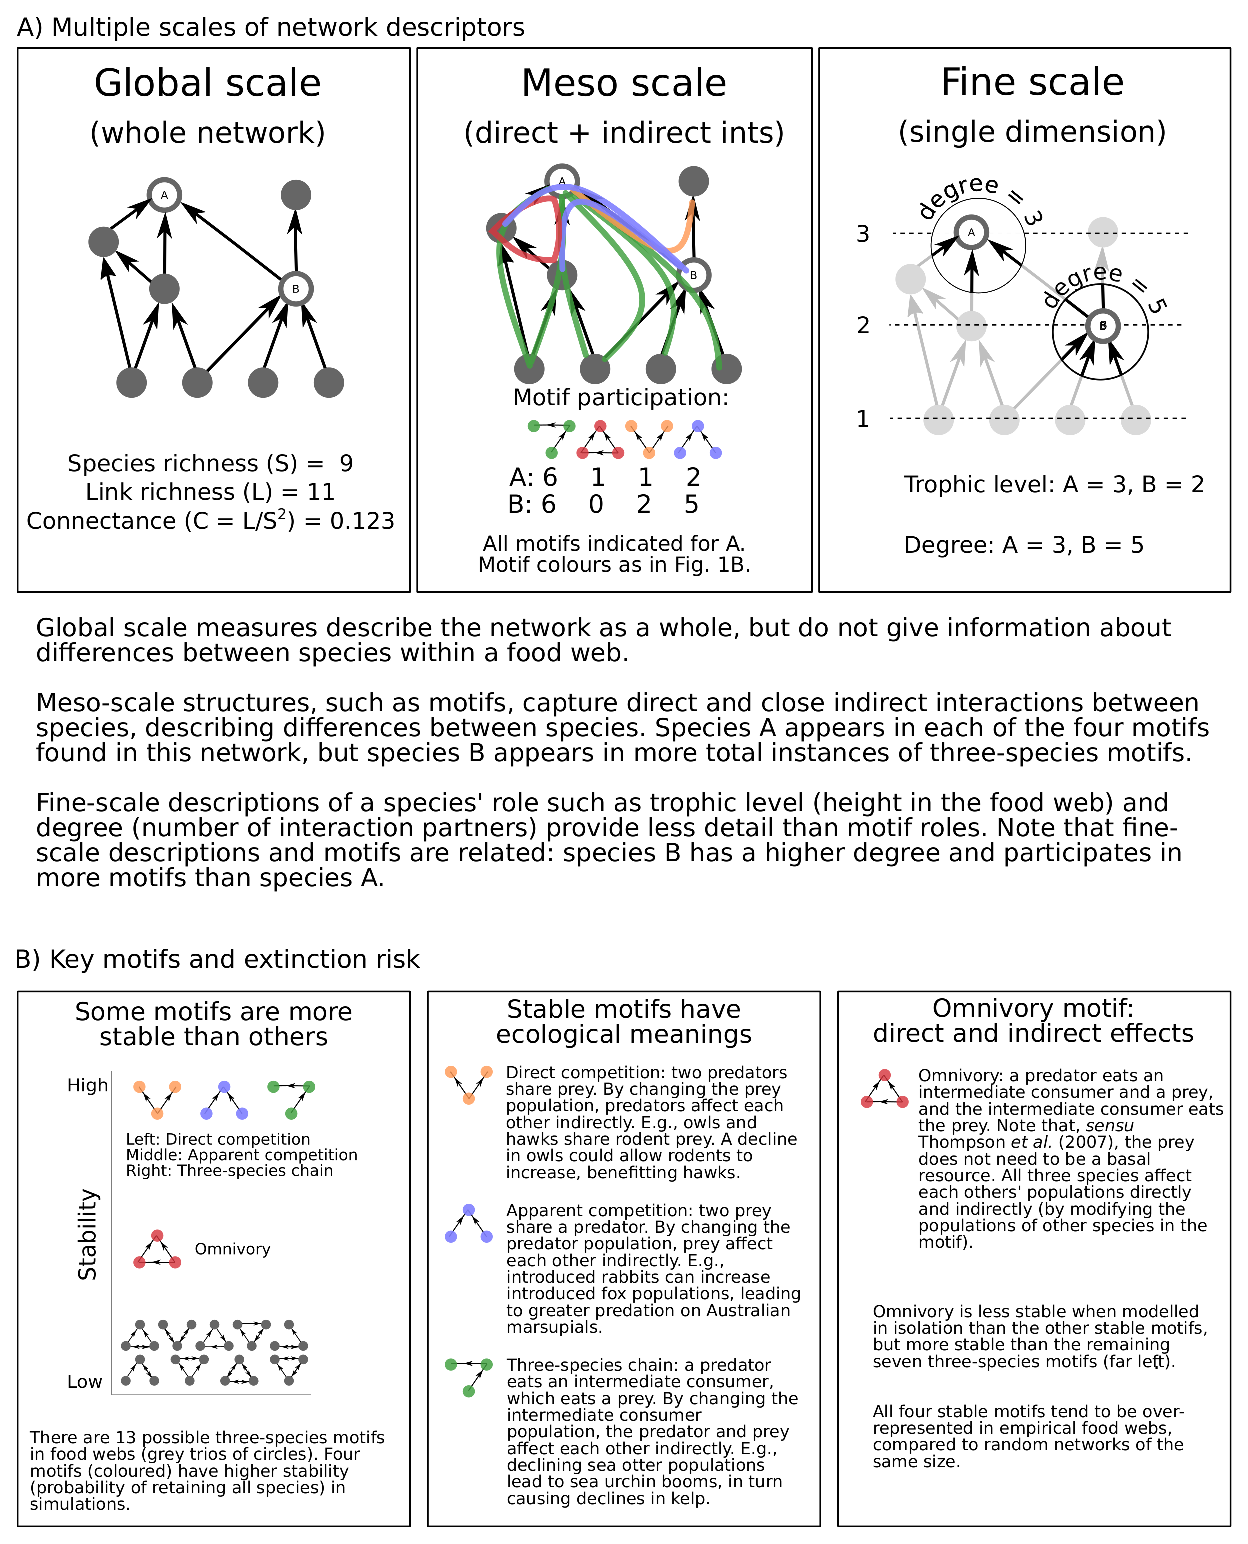
\includegraphics[width=.9\textwidth]{figures/motifs_box.eps}
        \caption{Figure 1.}
        \label{motifs}
    \end{figure}

    \clearpage

    \begin{figure}[h!]
        \centering
        \includegraphics{figures/roles/persistence_vs_degTL.eps}
        \caption{Mean persistence time increased with increasing degree for species at low trophic levels (STL 1-2) but decreased with increasing degree for species at high trophic levels (STL \textgreater2). The figure is based on the fixed effects in a regression of persistence against degree, trophic level, their interaction, and a random effect of global network structure.}
        \label{fig:persistence_degTL}
    \end{figure}

    \clearpage

    \begin{figure}[h!]
        \centering
        \includegraphics{figures/motifs_vs_DegTL.eps}
        \caption{Degree was strongly and significantly associated with motif participation, but trophic level was much more weakly, though still significantly, associated with motif participation (Appendix \emph{SX}). For each version of motif participation, we show the marginal effect of changes in participation in a single motif, holding participation in all other motifs constant at their mean values. For the species-normalised (frequency) motifs, which must sum to 1, this is an unrealistic simplification. }
        \label{fig:motifs_degTL}
    \end{figure}


\clearpage

\section*{Appendices}

\begin{spacing}{2.0}

All of the following Appendices are included as supplemental information.

    % \subsection*{S1: Testing consistence of times to extinction}
    
    %     Supplemental methods and results related to testing whether the identity of the removed species has a large effect on the time to extinction for non-removed species. Includes \textbf{Figure S1}.
    
    % \subsection*{S2: Details of PERMANOVA results}
        
    %     Supplemental results for PERMANOVAs testing whether species' overall roles are related to their mean times to exinction. Includes \textbf{Figure S2, Tables S1-S2}.
    
    % \subsection*{S3: Relating motifs roles to other measures}
        
    %     Gives the slopes of relationships between motif roles and degree or shortest trophic level (STL) in \textbf{Tables S3-S4}.
        
    % \subsection*{S4: Motif labels}
        
    %     \textbf{Figure S3} illustrates the 13 unique three-species motifs and labels each one according to the naming scheme in~\citet{Stouffer2007}.

\end{spacing}

\end{document}



